% Anonymous working draft, 2 October 2026.
% Evidence: completed four-dataset validation study and nonlearned baselines.
% The ongoing 36-condition extension is not part of the main comparison;
% its completed subset at the observation cutoff appears in Appendix A.
% PAKDD 2027 page limit has not yet been announced.
% Standalone source: figures and bibliography are embedded below.
\documentclass[runningheads]{llncs}
\usepackage[T1]{fontenc}
\usepackage{amsmath}
\usepackage{newtxtext}
\usepackage[varvw]{newtxmath}
\usepackage{booktabs,array}
\usepackage{tikz}
\usetikzlibrary{arrows.meta,positioning,fit,calc}
\usepackage[hidelinks]{hyperref}
\newcommand{\method}{TitanTPP}
\newcommand{\GELU}{\operatorname{GELU}}
\newcommand{\softplus}{\operatorname{softplus}}
\newcommand{\E}{\mathcal{E}}
\newcommand{\Hcal}{\mathcal{H}}
\definecolor{enc}{RGB}{226,237,248}
\definecolor{hist}{RGB}{218,239,231}
\definecolor{head}{RGB}{249,237,212}
\definecolor{ink}{RGB}{44,63,78}
\begin{document}
\title{TitanTPP: Efficient History Correction for Next-Event Quantity Prediction}
\titlerunning{TitanTPP: Efficient History Correction}
\author{Anonymous Authors}
\authorrunning{Anonymous Authors}
\institute{Anonymous Institution}
\maketitle

\begin{abstract}
Predicting demand events requires estimating both their timing and their
quantity from an irregular history. We introduce TitanTPP, a compact event
encoder with a bottleneck history correction between two causal attention
blocks. The correction combines current and immediately preceding contextual
states, while learned static banks supply additional context without online
parameter updates. A common-input, common-head comparison covers six temporal
point process encoders across four datasets and three seeds. On the development
validation partitions, TitanTPP reduces mean quantity RMSE by 15.85\% on Taxi
and 34.39\% on Intermittent relative to the strongest external encoder on each
dataset. The improvement over the last-quantity baseline on Intermittent is
smaller, at 2.04\% in RMSE, and that baseline achieves lower MAE. RAF exhibits
a small RMSE gain with an MAE trade-off, while Instacart favors external
encoders on RMSE. Matched batch measurements against a Titans-MAC adapter
indicate that the MAC adapter requires 5.58--5.74 times TitanTPP's
training-step compute time. TitanTPP reduces peak allocated training memory by
approximately 75.5\%, while its evaluation memory is higher. These results support compact history correction for next-event
quantity prediction and identify the demand settings in which its benefits
are strongest.
\keywords{Temporal point processes \and Event quantity prediction \and History encoding \and Intermittent demand}
\end{abstract}

\section{Introduction}
Demand planning concerns both the time of the next requirement and its size.
When observations are sporadic, a history of event gaps and quantities provides
a direct representation of those two quantities. Classical intermittent-demand
methods separate demand occurrence from size~\cite{croston1972forecasting}.
Neural renewal models extend this event-based perspective through learned
arrival and quantity distributions~\cite{turkmen2021renewal}. A useful event
encoder must preserve predictive relationships in the history while remaining
practical to train.

Attention combines information across events, and neural memory provides
another route for historical context. Titans integrates attention with a
memory module that adapts at test time~\cite{behrouz2025titans}. For bounded
event histories, a simpler question motivates our design: can a compact,
feed-forward correction exploit recent-event relationships without online
memory updates?

We propose \method, a causal encoder for next-event quantity and duration
prediction. Two attention blocks surround a bottleneck residual that relates
the current contextual state to its immediate observed predecessor. The first
block encodes the history; the correction exposes an explicit adjacent-state
interaction; the second block integrates the adjusted representations.
Learned persistent vectors and a static prototype bank complement this path.
The correction adds 6,144 parameters, and all learned parameters remain fixed
during inference.

Our evaluation separates quantity accuracy, duration likelihood, and
computational cost. Under shared inputs, prediction heads, and training rules,
\method\ improves quantity MAE and RMSE over six TPP encoders in every paired
seed on Taxi and Intermittent. The gains are smaller on RAF and do not extend
to the best Instacart RMSE. Simple quantity baselines further qualify the
Intermittent result: repeating the last quantity achieves lower MAE, whereas
\method\ achieves lower RMSE. Matched batch measurements provide a separate
comparison with a Titans-MAC event adapter.

Our contributions are as follows.
\begin{enumerate}
\item We introduce a compact event-history correction architecture that
combines adjacent contextual states between causal encoder blocks and retains
static memory access without online updates.
\item We evaluate next-event quantity prediction across four datasets and
three seeds, including six common-head TPP encoders, a correction-removal
control, and two nonlearned baselines. The results identify substantial gains
over the learned comparators on Taxi and Intermittent and quantify their
limits in other demand settings.
\item We characterize computational cost against a Titans-MAC adapter using
matched input batches. The measurements distinguish lower training compute
and memory from the higher allocation observed during evaluation.
\end{enumerate}

\section{Related Work}
\paragraph{Event-history encoders.}
Hawkes processes model event dependence through self-excitation and mutual
excitation~\cite{hawkes1971spectra}. Neural TPPs learn historical
representations and conditional event distributions~\cite{shchur2021review}.
RMTPP summarizes history with a recurrent network~\cite{du2016rmtpp}, and the
Neural Hawkes Process employs continuous-time LSTM states~\cite{mei2017nhp}.
THP, SAHP, and AttNHP encode temporal dependencies through
attention~\cite{zuo2020thp,zhang2020sahp,yang2022attnhp}.
S2P2 combines continuous-time state evolution with event impulses and
nonlinear transformations~\cite{chang2025s2p2}, drawing on HiPPO's
polynomial-projection framework~\cite{gu2020hippo}. We compare these encoder
families through a common numerical-input and prediction-head interface.

\paragraph{Event distributions and quantity forecasting.}
Neural TPPs can parameterize an integrated intensity~\cite{omi2019fully} or
directly specify a conditional duration distribution~\cite{shchur2020intensityfree}.
Our duration head follows the latter approach and evaluates the probability
mass of recorded integer durations. In demand forecasting, Croston-style
methods and their extensions separate occurrence from
size~\cite{croston1972forecasting,syntetos2005accuracy,teunter2011obsolescence}.
Deep renewal processes connect this decomposition to neural arrival-and-size
models~\cite{turkmen2021renewal}; FlexTPP models mixed event attributes with
distribution-specific heads~\cite{draxler2025flextpp}. These methods motivate
the joint study of numerical quantities and event timing.

DeepAR learns probabilistic forecasts across related
series~\cite{salinas2020deepar}. PatchTST and iTransformer explore temporal
patches and variate tokens, respectively~\cite{nie2023patchtst,liu2024itransformer}.
Their calendar-horizon formulations differ from our next-event target.
\method\ predicts the size and gap of a positive-demand event; demand
accumulated over a future calendar interval requires an additional event
aggregation procedure.

\paragraph{Residual correction and memory.}
Residual learning~\cite{he2016residual} and bottleneck
adapters~\cite{houlsby2019adapters} provide compact transformation paths.
\method\ specializes this structure to adjacent event representations and
trains it jointly with the encoder. Its zero output initialization initially
preserves the base function, sharing a motivation with zero-initialized
residual paths such as ReZero~\cite{bachlechner2021rezero}.
Memory networks retrieve learned context~\cite{sukhbaatar2015memory}, while
Titans updates a neural memory at test time~\cite{behrouz2025titans}.
Our design retains static retrieval and implements history correction through
ordinary feed-forward operations. The efficiency comparison evaluates these
complete computational paths.

\section{Method}
\subsection{Observed Events and Causal Encoding}
Let $\Hcal_n=\{(t_i,q_i)\}_{i=1}^{n}$ denote an observed event history,
with recorded inter-event durations $\Delta_i$ and quantities $q_i$.
We predict the next quantity and recorded duration. Each training window
contains an observed prefix and one target event. The target contributes to
the loss only; both heads read the last observed state.

For padded windows, $v_i$ indicates a valid row and $w_i$ indicates a permitted
observed row. With $o_i=v_iw_i$, the input embedding is
\begin{equation}
 f_i=[\log(1+\Delta_i),\log(1+q_i)]^\top,\qquad
 x_i=o_i(W_{\rm in}f_i+b_{\rm in}+p_i),
 \label{eq:input}
\end{equation}
where $p_i$ is a learned positional embedding and the hidden dimension is
$d=64$. Unobserved inputs are replaced by zero before the logarithm and
projection. Durations follow each dataset's recorded units, including the
loader's positive-gap convention for the first row.

The encoder contains two pre-normalized causal attention
blocks~\cite{vaswani2017attention,ba2016layernorm}. Each block has four heads
and a feed-forward width of 128. A learned bank $P^{(\ell)}\in\mathbb R^{16\times d}$
supplies persistent keys and values in block $\ell$. Suppressing head indices,
\begin{equation}
 \begin{aligned}
 K&=[P^{(\ell)};K_{\rm events}],\quad V=[P^{(\ell)};V_{\rm events}],\\
 A_i&=\operatorname{softmax}(Q_iK^\top/\sqrt{d_h}+C_i)V,
 \end{aligned}
 \label{eq:attention}
\end{equation}
where $d_h=16$ and the persistent bank denotes the corresponding head slice.
The mask $C_i$ permits all persistent vectors and only observed event keys at
positions $j\leq i$. The same raw bank vectors serve as keys and values.
Attention and GELU feed-forward transformations each have a residual path,
with dropout 0.1. Unobserved query states are zeroed after each residual.
Writing the blocks as $\E_1$ and $\E_2$, the first produces $H^{(1)}=\E_1(X)$.

\subsection{Bottleneck History Correction}
The intermediate correction explicitly relates the current contextual state
to its immediate observed predecessor. Let $\pi(i)$ denote that predecessor,
skipping padding, and let $c_i$ count observed rows since the latest withheld
valid row, including row $i$. For eight thresholds
$\tau=(1,2,4,8,16,32,64,128)$, branch availability is
\begin{equation}
 a_{i,b}=o_i\,\mathbf 1\{c_i>\tau_b\},\qquad b=1,\ldots,8.
 \label{eq:availability}
\end{equation}
Branch $b$ contains bias-free matrices $U_b\in\mathbb R^{4\times 2d}$ and
$V_b\in\mathbb R^{d\times4}$. Its output enters the residual
\begin{align}
 r_i&=\frac18\sum_{b=1}^{8}a_{i,b}V_b
       \GELU\bigl(U_b[h_i^{(1)};h_{\pi(i)}^{(1)}]\bigr),\label{eq:correction}\\
 \widetilde h_i^{(1)}&=h_i^{(1)}+r_i,\qquad
 H^{(2)}=\E_2(\widetilde H^{(1)}).\label{eq:insert}
\end{align}
GELU follows its exact error-function formulation~\cite{hendrycks2016gelu}.
All eight branches read the same immediate predecessor. The thresholds govern
availability, not retrieval lag. The divisor remains eight when fewer
branches are active. If no predecessor exists, all branches are unavailable
and $r_i=0$. Withheld valid rows reset correction eligibility; padding does
not. This rule leaves the encoder's causal attention history intact.

The correction adds $8(2dr+rd)=6{,}144$ parameters for bottleneck width $r=4$.
Every output matrix $V_b$ initializes to zero, so the correction initially
preserves the base encoder's function under the same stochastic state.
Parameter construction preserves the caller's random-number stream.
Both inputs in Eq.~\eqref{eq:correction} are contextual states, allowing the
correction to depend on information preceding the adjacent event pair.
Figure~\ref{fig:architecture} summarizes the resulting computation.

\begin{figure}[t]
\centering
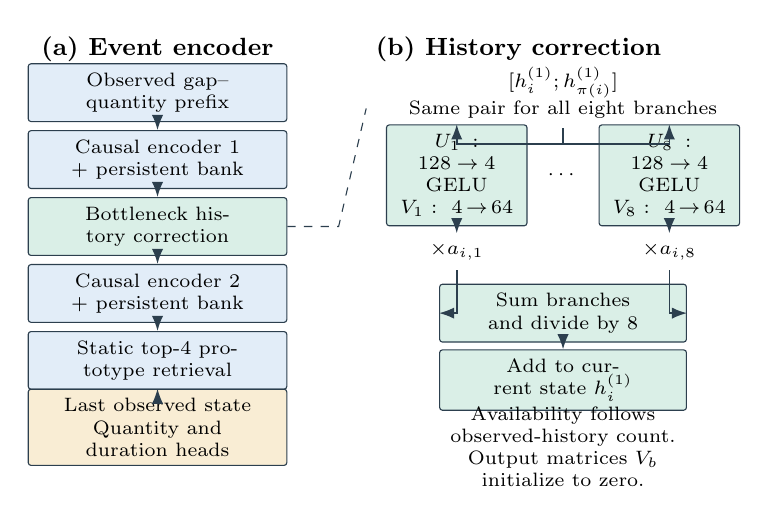
\begin{tikzpicture}[x=1cm,y=1cm,>=Latex,font=\scriptsize,
 block/.style={draw=ink,rounded corners=1pt,align=center,minimum height=.56cm,text width=3.05cm,fill=enc},
 arr/.style={->,draw=ink,line width=.55pt}]
\node[anchor=west,font=\small\bfseries] at (-1.6,.55) {(a) Event encoder};
\node[block] (in) at (0,0) {Observed gap--quantity prefix};
\node[block] (e1) at (0,-.85) {Causal encoder 1 + persistent bank};
\node[block,fill=hist] (corr) at (0,-1.7) {Bottleneck history correction};
\node[block] (e2) at (0,-2.55) {Causal encoder 2 + persistent bank};
\node[block] (ret) at (0,-3.4) {Static top-4 prototype retrieval};
\node[block,fill=head] (heads) at (0,-4.25) {Last observed state\\Quantity and duration heads};
\foreach \a/\b in {in/e1,e1/corr,corr/e2,e2/ret,ret/heads}{\draw[arr] (\a)--(\b);}
\node[anchor=west,font=\small\bfseries] at (2.65,.55) {(b) History correction};
\node[align=center] (pair) at (5.15,0) {$[h_i^{(1)};h_{\pi(i)}^{(1)}]$\\Same pair for all eight branches};
\node[block,text width=1.55cm,fill=hist] (b1) at (3.8,-1.05) {$U_1:\ 128\!\to\!4$\\GELU\\$V_1:\ 4\!\to\!64$};
\node[block,text width=1.55cm,fill=hist] (b8) at (6.5,-1.05) {$U_8:\ 128\!\to\!4$\\GELU\\$V_8:\ 4\!\to\!64$};
\node at (5.15,-1.05) {$\cdots$};
\node[align=center] (m1) at (3.8,-2.02) {$\times a_{i,1}$};
\node[align=center] (m8) at (6.5,-2.02) {$\times a_{i,8}$};
\node[block,text width=2.9cm,fill=hist] (sum) at (5.15,-2.8) {Sum branches and divide by 8};
\node[block,text width=2.9cm,fill=hist] (add) at (5.15,-3.65) {Add to current state $h_i^{(1)}$};
\draw[arr] (pair.south)--++(0,-.2)-|(b1.north);
\draw[arr] (pair.south)--++(0,-.2)-|(b8.north);
\draw[arr] (b1)--(m1);\draw[arr] (b8)--(m8);
\draw[arr] (m1.south)|-(sum.west);\draw[arr] (m8.south)|-(sum.east);
\draw[arr] (sum)--(add);
\draw[draw=ink,dashed] (corr.east)--(2.3,-1.7)--(2.65,-.2);
\node[align=center,text width=4.4cm] at (5.15,-4.5) {Availability follows observed-history count.\\Output matrices $V_b$ initialize to zero.};
\end{tikzpicture}
\Description{The left pipeline passes observed gaps and quantities through
two causal encoders with a history correction between them, then static
prototype retrieval and two prediction heads. The expanded module on the
right sends the same current and predecessor state pair through eight
independent bottleneck branches, applies availability masks, sums and divides
by eight, and adds the result to the current state.}
\caption{\method\ and the expanded correction. The eight branches share an
input pair but have separate parameters. The two persistent banks and final
prototype bank are learned during training and fixed during inference. The
next target event is withheld from the encoder.}
\label{fig:architecture}
\end{figure}

\subsection{Static Retrieval and Prediction Heads}
A bank $M\in\mathbb R^{64\times d}$ supplies static prototypes after the
second block. At each observed position, cosine similarity selects four
prototypes whose raw vectors enter an unweighted residual:
\begin{equation}
 \begin{aligned}
 S_i&=\operatorname{TopK}_{j,\,k=4}\operatorname{cos}(h_i^{(2)},m_j),\\
 z_i&=o_i\left(h_i^{(2)}+\frac14\sum_{j\in S_i}m_j\right).
 \end{aligned}
 \label{eq:retrieval}
\end{equation}
Normalization affects selection only. The bank ties keys and values and
receives no online writes. Both heads read $z_n$, the last observed state.

The quantity head predicts a nonnegative point estimate through
\begin{equation}
 \widehat y_{n+1}=\softplus(w_q^\top z_n+b_q),\qquad
 \widehat q_{n+1}=\exp(\widehat y_{n+1})-1.\label{eq:quantity}
\end{equation}
At initialization, $w_q=0$ and $b_q$ yields the training mean of
$\log(1+q)$. The duration head specifies a positive latent duration $T$:
\begin{equation}
 \begin{aligned}
 \mu_n&=w_\mu^\top z_n+b_\mu,\quad
 \sigma_n=\softplus(w_\sigma^\top z_n+b_\sigma)+10^{-3},\\
 \log(T/s)\mid\Hcal_n&\sim\mathcal N(\mu_n,\sigma_n^2).
 \end{aligned}
 \label{eq:duration}
\end{equation}
For recorded durations $D=\max(1,\operatorname{round}(T))$, with optional
upper coding at $K$, the probability mass is
\begin{equation}
 p(D=d\mid\Hcal_n)=
 \begin{cases}
 F_n(1.5),&d=1,\\
 1-F_n(K-0.5),&d=K\text{ under upper coding},\\
 F_n(d+0.5)-F_n(d-0.5),&\text{otherwise},
 \end{cases}\label{eq:mass}
\end{equation}
where $F_n$ is the lognormal CDF. Instacart has $K=30$; other datasets lack
upper coding. The scales $s$ are one hour, three weeks, seven days, and six
months for Taxi, Intermittent, Instacart, and RAF, respectively. Stable
float64 CDF or survival-function differences evaluate the log masses.

\subsection{Training and Selection}
The objective combines recorded-duration NLL and squared log-quantity error:
\begin{equation}
 \mathcal L=\frac1{|\mathcal B|}\sum_{n\in\mathcal B}
 \left[-\log p(D_{n+1}\mid\Hcal_n)
 +(\widehat y_{n+1}-\log(1+q_{n+1}))^2\right].\label{eq:loss}
\end{equation}
Each window contributes one final target, and the quantity term has unit
weight. AdamW~\cite{loshchilov2019adamw} optimizes the objective with learning
rate $10^{-3}$, weight decay 0.01, gradient clipping at norm 1, and batch size
128. Training permits at most 300 epochs, at least 40 epochs, and patience
40. We select the earliest checkpoint attaining the strictly lowest finite
validation RMSE on the raw quantity scale. MAE and duration NLL come from
that same checkpoint.

At fixed width and branch count, the correction requires linear projection
work in sequence length. The complete encoder retains the quadratic
interactions of causal attention. This distinction motivates measuring the
complete model rather than inferring its cost from the correction alone.

\section{Experimental Setup}
\subsection{Data and Evaluation Scope}
The four datasets encode different quantity-bearing events. Taxi counts
pickups within a spatial cell and an active hour. Intermittent contains
positive order quantities for site--part sequences. Instacart aggregates
product rows for each user on the same recorded activity day, yielding a
basket-size proxy rather than physical purchased units. RAF represents
positive monthly spare-parts demand, with event gaps measured in months.
Zero-demand calendar periods enter the gaps rather than separate quantity
targets. Table~\ref{tab:data} summarizes the target populations.

\begin{table}[t]
\caption{Frozen train and validation targets. Maximum rows include the
withheld target; lookbacks follow the dataset's recorded units.}
\label{tab:data}\centering\small
\begin{tabular}{lrrrl}
\toprule
Dataset & Train & Validation & Max. rows & Lookback\\
\midrule
Taxi & 38,393 & 8,268 & 256 & 168 hours\\
Intermittent & 393,824 & 86,285 & 256 & 520 weeks\\
Instacart & 1,991,192 & 503,733 & 64 & 52 days\\
RAF & 25,779 & 6,690 & 84 & 84 months\\
\bottomrule
\end{tabular}
\end{table}

Frozen splits follow event order within each sequence, approximately
70/15/15. The comparisons in this draft concern development validation
partitions, which also informed architecture choices. Taxi sequence
selection and Intermittent filtering depend on full observed sequence
lengths, defining retrospective cohorts. We distinguish these comparisons
from an independent final evaluation in Sect.~\ref{sec:limitations}.

\subsection{Comparators and Controls}
The common-head panel contains RMTPP, NHP, THP, SAHP, S2P2, and AttNHP.
Each receives the same gap--quantity history and target and connects to the
same quantity and duration heads. All follow Eq.~\eqref{eq:loss}, the same
optimizer settings, and the same checkpoint rule. This explicit interface
follows the reproducibility motivation of TPP benchmarking efforts such as
EasyTPP~\cite{xue2024easytpp}. Implementations employ
PyTorch~\cite{paszke2019pytorch}.

S2P2 retains HiPPO initialization, complex diagonal evolution, backward
zero-order-hold discretization, event impulses, relative time, and
normalization/nonlinearity. The adaptation has width 64, two layers, and
state size 16. Its affine-doubling recurrence was checked against the
sequential equations; it incurs $O(L\log L)$ work rather than the original
work-efficient scan. AttNHP retains query/context attention, sinusoidal time
encoding, and tanh query residuals, with width 64, two layers, one attention
head, time width 16, and no feed-forward sublayer. It queries the right limit
of the last observed event, without the next target time. Numerical input
projections and common heads replace the original categorical inputs and
native outputs.

The B control retains the causal encoder and learned banks but removes the
intermediate correction. It measures the effect of adding the history path,
including its parameters. An exploratory normalization variant divides by
the number of available branches instead of eight. We retain a single
representative \method\ architecture throughout the main comparison.

Two nonlearned baselines predict either the last observed quantity or the
mean quantity in exactly the same observed input window. They require no
training or seed averaging. Neither specifies a duration distribution, so
duration NLL is undefined for them.

\subsection{Metrics and Repeated Runs}
We report raw quantity MAE and RMSE, and recorded-duration NLL from
Eq.~\eqref{eq:mass}. RMSE selection assigns greater weight to large absolute
quantity errors; MAE records average absolute error. Comparisons remain
within each dataset because their quantity scales differ~\cite{hyndman2006accuracy}.
Duration NLL evaluates the probability assigned to the recorded observation
through the logarithmic score~\cite{gneiting2007proper}.

Learned models have three seeds, 42, 52, and 62. Tables report their arithmetic
means and sample standard deviations, and the analysis includes paired seeds.
The common-head panel contains 84 completed runs across 28 dataset--model
groups. Selected and last checkpoints, validation re-evaluations, and source
identities are retained. All three metrics refer to the RMSE-selected
checkpoint rather than separate metric-specific minima.

\section{Results}
\subsection{Comparison with TPP Encoders}
Table~\ref{tab:main} reports the complete four-dataset comparison. On Taxi
and Intermittent, \method\ achieves lower quantity MAE and RMSE than each
external encoder in all 36 paired comparisons (two datasets, six comparators,
three seeds). RMTPP is the strongest external model on the mean quantity
metrics for both datasets. Relative to RMTPP, \method\ reduces MAE/RMSE by
10.13\%/15.85\% on Taxi and 21.72\%/34.39\% on Intermittent. Several encoders
achieve better duration NLL, so quantity and timing rankings differ.

\begin{table}[p]
\caption{Development validation results, mean $\pm$ sample standard
deviation over three seeds. All metrics come from the same RMSE-selected
checkpoint. Bold denotes the lowest mean within each dataset and metric in
this common-head panel; the nonlearned baselines appear separately.}
\label{tab:main}\centering\small
\begin{tabular}{lrrr}
\toprule
Model & Quantity MAE & Quantity RMSE & Time NLL\\
\midrule
\multicolumn{4}{l}{\textit{Taxi}}\\
TitanTPP & $\mathbf{25.6237\pm0.8320}$ & $\mathbf{79.7111\pm2.8260}$ & $1.0387\pm0.2843$\\
RMTPP & $28.5124\pm0.6344$ & $94.7283\pm3.4006$ & $1.5798\pm0.9400$\\
THP & $32.4095\pm0.8144$ & $107.5977\pm4.5040$ & $0.6629\pm0.0174$\\
NHP & $94.2694\pm1.8752$ & $318.8148\pm5.3011$ & $\mathbf{0.6516\pm0.0021}$\\
SAHP & $34.2260\pm0.4539$ & $120.5273\pm1.9996$ & $0.6848\pm0.0146$\\
S2P2 & $33.0231\pm0.5569$ & $106.3540\pm1.9135$ & $0.6658\pm0.0242$\\
AttNHP & $35.9811\pm1.6088$ & $127.1290\pm8.9919$ & $0.6876\pm0.0194$\\
\midrule
\multicolumn{4}{l}{\textit{Intermittent}}\\
TitanTPP & $\mathbf{0.7005\pm0.0541}$ & $\mathbf{1.6730\pm0.0819}$ & $0.4971\pm0.2095$\\
RMTPP & $0.8949\pm0.0494$ & $2.5499\pm0.1604$ & $0.2748\pm0.0047$\\
THP & $0.8993\pm0.0661$ & $2.7534\pm0.1784$ & $0.2911\pm0.0045$\\
NHP & $4.5188\pm0.1706$ & $12.8755\pm1.0405$ & $0.4613\pm0.0969$\\
SAHP & $1.8619\pm0.0899$ & $7.0298\pm0.7673$ & $0.3448\pm0.0138$\\
S2P2 & $0.9359\pm0.0086$ & $2.5758\pm0.0766$ & $\mathbf{0.2349\pm0.0189}$\\
AttNHP & $1.0413\pm0.0938$ & $3.0799\pm0.2982$ & $0.2946\pm0.0569$\\
\midrule
\multicolumn{4}{l}{\textit{RAF}}\\
TitanTPP & $9.2506\pm0.0855$ & $\mathbf{33.9507\pm0.0588}$ & $3.5446\pm0.0669$\\
RMTPP & $\mathbf{9.1362\pm0.0557}$ & $34.5503\pm0.2506$ & $3.5191\pm0.1463$\\
THP & $9.3014\pm0.1819$ & $34.7445\pm0.3204$ & $3.3928\pm0.0187$\\
NHP & $9.1793\pm0.0882$ & $36.2731\pm0.3186$ & $\mathbf{3.3889\pm0.0556}$\\
SAHP & $9.2332\pm0.0209$ & $35.4193\pm0.2130$ & $3.7415\pm0.0745$\\
S2P2 & $9.2730\pm0.0517$ & $33.9947\pm0.1261$ & $3.4187\pm0.0284$\\
AttNHP & $9.1917\pm0.0434$ & $34.8766\pm0.0676$ & $3.9707\pm0.0609$\\
\midrule
\multicolumn{4}{l}{\textit{Instacart}}\\
TitanTPP & $3.9916\pm0.0026$ & $5.8827\pm0.0048$ & $2.8071\pm0.0041$\\
RMTPP & $\mathbf{3.9852\pm0.0052}$ & $5.8775\pm0.0213$ & $2.8051\pm0.0048$\\
THP & $4.0013\pm0.0025$ & $5.8582\pm0.0253$ & $2.8056\pm0.0016$\\
NHP & $4.4923\pm0.0304$ & $6.7613\pm0.0538$ & $2.8132\pm0.0080$\\
SAHP & $3.9979\pm0.0099$ & $5.8776\pm0.0067$ & $2.8018\pm0.0013$\\
S2P2 & $3.9987\pm0.0063$ & $\mathbf{5.8523\pm0.0150}$ & $\mathbf{2.7970\pm0.0014}$\\
AttNHP & $3.9958\pm0.0021$ & $5.8648\pm0.0194$ & $2.8080\pm0.0028$\\
\bottomrule
\end{tabular}
\end{table}

On RAF, \method's mean RMSE of 33.9507 is close to S2P2's 33.9947, a 0.13\%
difference. \method\ leads in two of three paired seeds. RMTPP achieves lower
MAE, 9.1362 versus 9.2506, and NHP achieves lower time NLL. The result
extends the evaluation to spare-parts demand while exposing a metric-dependent
trade-off.

On Instacart, RMTPP has the lowest mean MAE, while S2P2 has the lowest RMSE
and time NLL. \method's MAE is 0.16\% higher than RMTPP's. Relative to S2P2
and AttNHP, \method\ reduces mean MAE by 0.18\% and 0.11\%, respectively,
but increases mean RMSE by 0.52\% and 0.31\%. Both added comparators achieve
lower RMSE in every paired seed. The improvement observed on Taxi and
Intermittent therefore does not transfer uniformly to basket-size prediction.

\subsection{Comparison with Simple Quantity Rules}
Table~\ref{tab:naive} places the learned-model results beside two direct
history summaries. \method\ improves both quantity metrics over both rules
on Taxi, Instacart, and RAF. Intermittent is different. Repeating the last
quantity achieves MAE 0.5647, below \method's 0.7005, while \method\ reduces
RMSE from 1.7078 to 1.6730, a 2.04\% improvement. Thus the large gain over
the TPP encoder panel does not imply a similarly large gain over a simple
quantity predictor.

\begin{table}[t]
\caption{Nonlearned quantity rules on the same validation targets and
observed windows. \method\ entries are three-seed means; deterministic rules
have one result and no seed standard deviation or duration NLL.}
\label{tab:naive}\centering\small
\begin{tabular}{llrr}
\toprule
Dataset & Predictor & MAE & RMSE\\
\midrule
Taxi & TitanTPP & 25.6237 & 79.7111\\
 & Last quantity & 41.1951 & 134.3931\\
 & Window mean & 120.3771 & 368.7843\\
\midrule
Intermittent & TitanTPP & 0.7005 & 1.6730\\
 & Last quantity & 0.5647 & 1.7078\\
 & Window mean & 4.5537 & 13.7821\\
\midrule
Instacart & TitanTPP & 3.9916 & 5.8827\\
 & Last quantity & 4.9674 & 7.3473\\
 & Window mean & 4.0507 & 5.9030\\
\midrule
RAF & TitanTPP & 9.2506 & 33.9507\\
 & Last quantity & 11.3136 & 44.5742\\
 & Window mean & 10.8564 & 36.8499\\
\bottomrule
\end{tabular}
\end{table}

The Intermittent comparison also clarifies the role of the checkpoint
criterion. RMSE and MAE express different error priorities. A predictor can
reduce large squared errors while increasing average absolute error, and the
reported comparison preserves that distinction instead of selecting a
different checkpoint for each metric.

\subsection{Effect of the History Correction}
Removing the correction yields the B control in Table~\ref{tab:ablation}.
Adding the 6,144-parameter path reduces mean MAE/RMSE by 10.89\%/11.93\% on
Taxi and 7.68\%/6.04\% on Intermittent. On Instacart, MAE falls by about
0.04\% and RMSE rises by about 0.05\%. Mean time NLL increases on all three
datasets. The correction benefits quantity accuracy most in the same two
datasets that exhibit the largest gains over the external encoders.

\begin{table}[t]
\caption{Correction-removal control, mean $\pm$ sample standard deviation
over three seeds. B retains the causal encoder and both types of learned
bank, but omits the intermediate correction.}
\label{tab:ablation}\centering\small
\begin{tabular}{lrrr}
\toprule
Model & MAE & RMSE & Time NLL\\
\midrule
\multicolumn{4}{l}{\textit{Taxi}}\\
B & $28.7545\pm0.4526$ & $90.5093\pm0.5207$ & $0.7247\pm0.0668$\\
TitanTPP & $25.6237\pm0.8320$ & $79.7111\pm2.8260$ & $1.0387\pm0.2843$\\
\midrule
\multicolumn{4}{l}{\textit{Intermittent}}\\
B & $0.7588\pm0.0658$ & $1.7806\pm0.0439$ & $0.3846\pm0.1034$\\
TitanTPP & $0.7005\pm0.0541$ & $1.6730\pm0.0819$ & $0.4971\pm0.2095$\\
\midrule
\multicolumn{4}{l}{\textit{Instacart}}\\
B & $3.9932\pm0.0018$ & $5.8796\pm0.0166$ & $2.8065\pm0.0045$\\
TitanTPP & $3.9916\pm0.0026$ & $5.8827\pm0.0048$ & $2.8071\pm0.0041$\\
\bottomrule
\end{tabular}
\end{table}

An exploratory normalization variant replaces the fixed divisor in
Eq.~\eqref{eq:correction} with the number of available branches, with a
minimum divisor of one. On RAF, its three-seed MAE is $9.2322\pm0.0974$,
RMSE is $33.8979\pm0.0804$, and time NLL is $3.5631\pm0.0978$.
Relative to the representative model, MAE and RMSE fall by 0.20\% and
0.16\%, while time NLL rises. Each quantity metric improves in two of three
seeds. Seed-42 comparisons improve quantity error on Taxi but worsen it on
Intermittent. We treat this as structural sensitivity rather than choosing a
different representative architecture for each dataset.

\subsection{Where the Quantity Gains Occur}
Instacart's quantity strata explain the MAE--RMSE reversal against S2P2.
Targets at most 20 account for 89.37\% of its validation set. \method\ has
lower mean MAE and RMSE in both corresponding bins, while S2P2 performs
better in all three bins above 20. Above 35, mean RMSE is 24.6419 for
\method\ and 23.4686 for S2P2. Larger squared errors on high-quantity
targets outweigh the smaller-quantity gains in the aggregate RMSE.

Training-data characteristics offer a possible explanation for the dataset
differences. Instacart has a median usable history of five events. The
correlation between adjacent log quantities after subtracting each user's
mean is 0.037, compared with 0.749 on Taxi and 0.928 on Intermittent.
Short histories and weak adjacent association may limit the additional
information available to the correction. These descriptive associations
motivate the interpretation without identifying a causal mechanism.

\section{Computational Efficiency}
\subsection{Matched Measurement Protocol}
We compare \method\ with a Titans-MAC event adapter on identical RTX 5080
input batches for Taxi and Intermittent. Each configuration has length 256
and batch size 128. Each of three repetitions contains five warm-up batches
and 32 measured batches. GPU synchronization bounds compute timing;
within-repetition medians are summarized by their mean and sample standard
deviation across repetitions. Peak allocated and reserved memory counters
are reset after warm-up. Evaluation includes target-loss computation. The
runtime employs Python 3.12.13, PyTorch 2.11.0+cu130, CUDA 13.0, float32
model computation, disabled TF32, and deterministic execution settings.
Training timing includes forward and backward computation, loss evaluation,
gradient clipping, and the outer optimizer update; host-to-device transfer
is excluded. The MAC adapter retains observed-history memory updates and
a fixed-shape compiled scan. No new compiled graphs appear during measured
batches, and model order reverses in the second repetition.

\subsection{Time and Memory}
Table~\ref{tab:cost} reports synchronized per-batch compute times. The
MAC/TitanTPP ratio is 5.58--5.74 for training steps and 8.21--8.49 for
evaluation batches. These are matched batch-computation measurements, not
time-to-convergence estimates.

\begin{table}[t]
\caption{Compute time in milliseconds per batch, mean $\pm$ sample
standard deviation over three repetition medians. Ratios are paired within
repetition.}
\label{tab:cost}\centering\small
\begin{tabular}{llrrr}
\toprule
Dataset & Path & TitanTPP & MAC & MAC/TitanTPP\\
\midrule
Taxi & Train & $31.447\pm0.106$ & $180.582\pm6.056$ & $5.74\pm0.18$\\
 & Eval. & $7.632\pm0.009$ & $64.827\pm0.622$ & $8.49\pm0.08$\\
Intermittent & Train & $32.157\pm0.023$ & $179.472\pm0.555$ & $5.58\pm0.01$\\
 & Eval. & $7.909\pm0.030$ & $64.916\pm0.645$ & $8.21\pm0.07$\\
\bottomrule
\end{tabular}
\end{table}

\method\ reduces peak allocated training memory from about 7,631 MiB to
1,870 MiB, approximately 75.5\%. Evaluation reverses the allocation ordering:
389.2 MiB for \method\ versus 97.8 MiB for MAC, approximately 3.98 times
as much. Figure~\ref{fig:memory} contrasts the two paths.
Peak reserved training memory is 2,042.0 MiB for \method\ versus
7,670.0/7,646.0 MiB for MAC on Taxi/Intermittent. Evaluation reservations
are 416.0 MiB versus 151.3/130.0 MiB. The configured length-256 models
contain 96,003 and 122,310 trainable parameters, respectively.

\begin{figure}[t]
\centering
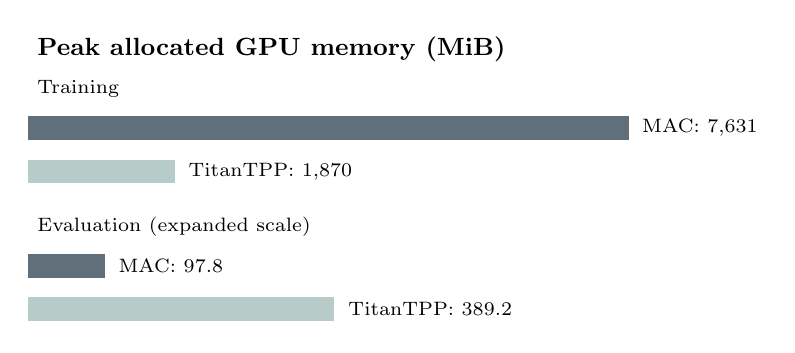
\begin{tikzpicture}[x=1cm,y=1cm,font=\scriptsize]
\node[font=\small\bfseries,anchor=west] at (0,2.9) {Peak allocated GPU memory (MiB)};
\node[anchor=west] at (0,2.4) {Training};
\fill[ink!75] (0,1.75) rectangle (7.631,2.05);
\node[anchor=west] at (7.68,1.9) {MAC: 7,631};
\fill[hist!80!ink] (0,1.2) rectangle (1.8695,1.5);
\node[anchor=west] at (1.92,1.35) {TitanTPP: 1,870};
\node[anchor=west] at (0,.65) {Evaluation (expanded scale)};
\fill[ink!75] (0,0) rectangle (.978,.3);
\node[anchor=west] at (1.03,.15) {MAC: 97.8};
\fill[hist!80!ink] (0,-.55) rectangle (3.892,-.25);
\node[anchor=west] at (3.95,-.4) {TitanTPP: 389.2};
\end{tikzpicture}
\Description{Two paired horizontal bar panels compare allocated GPU memory.
Training uses about 7631 MiB for MAC and 1870 MiB for TitanTPP. Evaluation
uses 97.8 MiB for MAC and 389.2 MiB for TitanTPP. The evaluation panel has an
expanded scale and all bars carry numeric labels.}
\caption{Mean peak allocated memory under matched batches. Taxi values
are plotted; Intermittent has the same TitanTPP values and a MAC training
allocation of 7,631.0 MiB instead of 7,631.3 MiB. Training and evaluation
panels have different horizontal scales; numeric labels preserve the
comparison.}
\label{fig:memory}
\end{figure}

These measurements support an efficient training path for the tested
configuration. Their scope is the complete backbone implementation, so the
time difference cannot be attributed solely to removing online memory
updates. The higher evaluation allocation also motivates reporting memory
separately for training and evaluation.

\section{Discussion and Limitations}\label{sec:limitations}
The results favor compact history correction for quantity prediction on Taxi
and Intermittent, with smaller or reversed gains elsewhere. The last-quantity
baseline's lower Intermittent MAE is particularly informative: outperforming
the learned encoder panel does not establish superiority over every useful
demand predictor. Duration likelihood also follows a different ranking.
The model is therefore best characterized through its quantity--timing--cost
trade-offs across demand settings.

The reported partitions informed architecture development. An independent
final evaluation still requires frozen model choices, an explicitly justified
evaluation population, and uncertainty procedures. Prior access to legacy
test artifacts prevents treating those data as automatically untouched.
Three-seed means, sample standard deviations, and paired wins describe
repeatability; they do not constitute a significance test.

The B comparison changes capacity as well as the correction path. It does
not isolate the individual effects of bottleneck rank, insertion position,
availability thresholds, or initialization. Parameter-matched current-state
controls, all-available-branch controls, and an event-native Deep Renewal
comparison are part of an ongoing extension and are outside the completed
four-dataset panel reported here. Appendix~\ref{app:extension} records the
completed subset available at this draft's observation cutoff, including
unfavorable results. The current results do not establish that
every design choice is necessary or optimal. Likewise, the static-retrieval
removal comparison available for a different internal variant does not
isolate that component's necessity in the representative architecture.

The common-head panel compares numerical-input adaptations of six TPP
encoders. Its objective and epoch cap do not equalize parameter counts,
tuning opportunity, or runtime. Rankings therefore concern these adapters.
The quantity head supplies a point estimate rather than a normalized quantity
density, and Eq.~\eqref{eq:loss} is a multi-task objective rather than a full
joint marked-event likelihood.

The data also limit prospective and operational interpretations. Cohorts are
retrospectively selected; Instacart is a basket-size proxy with upper-coded
durations; and the local Intermittent source still requires upstream
provenance and redistribution documentation. Inputs omit item identities,
calendar covariates, and product composition. The task addresses the next
recorded event, not inventory cost or accumulated calendar-horizon demand.
Finally, the efficiency study covers short, warmed batch workloads on one
GPU. Full-epoch time, time to matched accuracy, energy, and deployment
latency require separate measurements.

\section{Conclusion}
\method\ adds a compact bottleneck correction of adjacent contextual states
to a causal event encoder. Static learned banks complement this history
path while parameters remain fixed during inference. A four-dataset,
three-seed validation study identifies the strongest quantity gains over
the common-head TPP panel on Taxi and Intermittent. RAF and Instacart expose
smaller gains and metric-dependent reversals, and a last-quantity baseline
narrows the Intermittent advantage to RMSE.

Matched batch measurements indicate lower training-step compute time and
peak allocated training memory than a Titans-MAC adapter, alongside higher
evaluation memory. Together, the results support compact history correction
as a practical architecture for next-event quantity prediction. Completing
the structural comparisons and an independent final evaluation will clarify
how its benefits extend beyond the development partitions.

\appendix
\section{Completed Subset of the Ongoing Extension}\label{app:extension}
The following development results were available at the 2 October 2026,
07:14 KST observation cutoff. They extend the four-dataset comparison with
parameter-matched structural controls and a native quantity model. The
reported runs have completed training and selected/last validation
re-evaluation; their archived checkpoints await verification. These
preliminary results cover complete Taxi groups and two additional seed-42
conditions.

The current-only control removes the explicit predecessor input from the
correction while retaining history in the causal encoder. Its eight
64--6--64 branches match the original correction's 6,144 parameters and
retain the availability thresholds and fixed divisor. The all-available
control retains the original current--predecessor inputs and branch widths,
but activates all eight branches wherever a predecessor exists, still
dividing by eight. It differs from active-count normalization, which changes
the divisor rather than availability.

The Deep Renewal comparison is an event-native adapter with raw gap--quantity
inputs, two 64-unit LSTM layers, and shifted negative-binomial duration and
quantity distributions. It retains its native two-NLL objective rather than
the common quantity-regression loss. Input windows, targets, optimizer,
maximum epochs, and RMSE checkpoint selection follow the shared protocol.
It is a next-event adaptation, not a replication of calendar-horizon
forecasting experiments.

\begin{table}[h]
\caption{Completed Taxi groups from the ongoing extension, three-seed
validation mean $\pm$ sample standard deviation. The original MLP is reused.
The new conditions are preliminary pending archived-checkpoint verification.}
\label{tab:extension}\centering\small
\begin{tabular}{lrrr}
\toprule
Configuration & MAE & RMSE & Time NLL\\
\midrule
Original MLP & $25.624\pm0.832$ & $79.711\pm2.826$ & $1.039\pm0.284$\\
Current-only & $28.813\pm0.469$ & $90.048\pm1.513$ & $0.882\pm0.183$\\
All-available & $25.329\pm0.295$ & $78.121\pm0.711$ & $1.191\pm0.354$\\
Deep Renewal & $91.475\pm1.047$ & $404.786\pm2.978$ & $0.790\pm0.016$\\
\bottomrule
\end{tabular}
\end{table}

On Taxi, the original MLP improves mean MAE/RMSE over current-only by
11.07\%/11.48\%, with lower quantity errors in every paired seed.
All-available improves mean MAE/RMSE over the original by 1.15\%/1.99\%,
but increases mean time NLL; its MAE and RMSE gains occur in one and two
of the three paired seeds, respectively. Thus the available evidence
supports explicit predecessor correction without establishing that the
original availability thresholds are optimal. Deep Renewal has larger
quantity errors and lower time NLL in this setting. All three selected
checkpoints are at epoch 300, so the comparison reflects the budget endpoint
rather than a demonstrated convergence limit.

Two additional current-only seed-42 conditions are complete. On Intermittent,
current-only MAE/RMSE/time NLL are 0.74519/1.77305/0.35229, versus
0.63848/1.57849/0.34683 for the original MLP at the same seed. On Instacart,
the corresponding values are 3.99002/5.87224/2.80332 versus
3.99150/5.87873/2.80322. Instacart's small quantity difference favors
current-only, providing a counterexample to a universal benefit from the
explicit predecessor input. The all-available Intermittent and Instacart
seed-42 fits are in progress, and RAF extension fits have not started.
No three-seed conclusion is drawn for these incomplete groups.

\begin{thebibliography}{32}
\bibitem{paszke2019pytorch}
Paszke, A., Gross, S., Massa, F., Lerer, A., Bradbury, J., Chanan, G., et al.: \href{https://proceedings.neurips.cc/paper/2019/hash/bdbca288fee7f92f2bfa9f7012727740-Abstract.html}{PyTorch: An Imperative Style, High-Performance Deep Learning Library}. Advances in Neural Information Processing Systems 32 (2019).

\bibitem{hawkes1971spectra}
Hawkes, A. G.: \href{https://academic.oup.com/biomet/article-abstract/58/1/83/224809}{Spectra of some self-exciting and mutually exciting point processes}. Biometrika \textbf{58}(1), 83--90 (1971). \doi{10.1093/biomet/58.1.83}

\bibitem{gu2020hippo}
Gu, A., Dao, T., Ermon, S., Rudra, A., R\'{e}, C.: \href{https://proceedings.neurips.cc/paper/2020/hash/102f0bb6efb3a6128a3c750dd16729be-Abstract.html}{HiPPO: Recurrent Memory with Optimal Polynomial Projections}. Advances in Neural Information Processing Systems 33 (2020).

\bibitem{behrouz2025titans}
Behrouz, A., Zhong, P., Mirrokni, V.: \href{https://papers.nips.cc/paper_files/paper/2025/hash/a4ca07aa108036f80cbb5b82285fd4b1-Abstract-Conference.html}{Titans: Learning to Memorize at Test Time}. Advances in Neural Information Processing Systems 38, 125925--125962 (2025). \doi{10.52202/085713-3786}

\bibitem{turkmen2021renewal}
T\"{u}rkmen, A. C., Januschowski, T., Wang, Y., Cemgil, A. T.: \href{https://journals.plos.org/plosone/article?id=10.1371/journal.pone.0259764}{Forecasting intermittent and sparse time series: A unified probabilistic framework via deep renewal processes}. PLOS ONE \textbf{16}(11), e0259764 (2021). \doi{10.1371/journal.pone.0259764}

\bibitem{syntetos2005accuracy}
Syntetos, A. A., Boylan, J. E.: \href{https://www.sciencedirect.com/science/article/pii/S0169207004000792}{The accuracy of intermittent demand estimates}. International Journal of Forecasting \textbf{21}(2), 303--314 (2005). \doi{10.1016/j.ijforecast.2004.10.001}

\bibitem{vaswani2017attention}
Vaswani, A., Shazeer, N., Parmar, N., Uszkoreit, J., Jones, L., Gomez, A. N., et al.: \href{https://proceedings.neurips.cc/paper/2017/hash/3f5ee243547dee91fbd053c1c4a845aa-Abstract.html}{Attention Is All You Need}. Advances in Neural Information Processing Systems 30 (2017).

\bibitem{yang2022attnhp}
Yang, C., Mei, H., Eisner, J.: \href{https://openreview.net/forum?id=Rty5g9imm7H}{Transformer Embeddings of Irregularly Spaced Events and Their Participants}. International Conference on Learning Representations (2022).

\bibitem{hendrycks2016gelu}
Hendrycks, D., Gimpel, K.: \href{https://arxiv.org/abs/1606.08415}{Gaussian Error Linear Units (GELUs)}. arXiv:1606.08415 (2016).

\bibitem{salinas2020deepar}
Salinas, D., Flunkert, V., Gasthaus, J., Januschowski, T.: \href{https://www.sciencedirect.com/science/article/pii/S0169207019301888}{DeepAR: Probabilistic forecasting with autoregressive recurrent networks}. International Journal of Forecasting \textbf{36}(3), 1181--1191 (2020). \doi{10.1016/j.ijforecast.2019.07.001}

\bibitem{draxler2025flextpp}
Draxler, F., Meng, Y., Nelson, K., Laskowski, L., Yang, Y., Karaletsos, T., et al.: \href{https://proceedings.nips.cc/paper_files/paper/2025/hash/a6c7515ac435277dc92b75a07bb2257c-Abstract-Conference.html}{Transformers for Mixed-type Event Sequences}. Advances in Neural Information Processing Systems 38, 127441--127473 (2025). \doi{10.52202/085713-3833}

\bibitem{mei2017nhp}
Mei, H., Eisner, J.: \href{https://papers.nips.cc/paper_files/paper/2017/hash/6463c88460bd63bbe256e495c63aa40b-Abstract.html}{The Neural Hawkes Process: A Neurally Self-Modulating Multivariate Point Process}. Advances in Neural Information Processing Systems 30 (2017).

\bibitem{houlsby2019adapters}
Houlsby, N., Giurgiu, A., Jastrzebski, S., Morrone, B., De Laroussilhe, Q., Gesmundo, A., et al.: \href{https://proceedings.mlr.press/v97/houlsby19a.html}{Parameter-Efficient Transfer Learning for NLP}. Proceedings of the 36th International Conference on Machine Learning \textbf{97}, 2790--2799 (2019).

\bibitem{loshchilov2019adamw}
Loshchilov, I., Hutter, F.: \href{https://openreview.net/forum?id=Bkg6RiCqY7}{Decoupled Weight Decay Regularization}. International Conference on Learning Representations (2019).

\bibitem{croston1972forecasting}
Croston, J. D.: \href{https://link.springer.com/article/10.1057/jors.1972.50}{Forecasting and Stock Control for Intermittent Demands}. Journal of the Operational Research Society \textbf{23}(3), 289--303 (1972). \doi{10.1057/jors.1972.50}

\bibitem{ba2016layernorm}
Ba, J. L., Kiros, J. R., Hinton, G. E.: \href{https://arxiv.org/abs/1607.06450}{Layer Normalization}. arXiv:1607.06450 (2016).

\bibitem{he2016residual}
He, K., Zhang, X., Ren, S., Sun, J.: \href{https://openaccess.thecvf.com/content_cvpr_2016/html/He_Deep_Residual_Learning_CVPR_2016_paper.html}{Deep Residual Learning for Image Recognition}. Proceedings of the IEEE Conference on Computer Vision and Pattern Recognition, 770--778 (2016). \doi{10.1109/CVPR.2016.90}

\bibitem{du2016rmtpp}
Du, N., Dai, H., Trivedi, R., Upadhyay, U., Gomez-Rodriguez, M., Song, L.: \href{https://www.kdd.org/kdd2016/papers/files/rpp1081-duA.pdf}{Recurrent Marked Temporal Point Processes: Embedding Event History to Vector}. Proceedings of the 22nd ACM SIGKDD International Conference on Knowledge Discovery and Data Mining, 1555--1564 (2016). \doi{10.1145/2939672.2939875}

\bibitem{shchur2020intensityfree}
Shchur, O., Bilo\v{s}, M., G\"{u}nnemann, S.: \href{https://openreview.net/forum?id=HygOjhEYDH}{Intensity-Free Learning of Temporal Point Processes}. International Conference on Learning Representations (2020).

\bibitem{shchur2021review}
Shchur, O., T\"{u}rkmen, A. C., Januschowski, T., G\"{u}nnemann, S.: \href{https://www.ijcai.org/proceedings/2021/623}{Neural Temporal Point Processes: A Review}. Proceedings of the Thirtieth International Joint Conference on Artificial Intelligence, 4585--4593 (2021). \doi{10.24963/ijcai.2021/623}

\bibitem{zhang2020sahp}
Zhang, Q., Lipani, A., Kirnap, O., Yilmaz, E.: \href{https://proceedings.mlr.press/v119/zhang20q.html}{Self-Attentive Hawkes Process}. Proceedings of the 37th International Conference on Machine Learning \textbf{119}, 11183--11193 (2020).

\bibitem{hyndman2006accuracy}
Hyndman, R. J., Koehler, A. B.: \href{https://doi.org/10.1016/j.ijforecast.2006.03.001}{Another look at measures of forecast accuracy}. International Journal of Forecasting \textbf{22}(4), 679--688 (2006). \doi{10.1016/j.ijforecast.2006.03.001}

\bibitem{teunter2011obsolescence}
Teunter, R. H., Syntetos, A. A., Babai, M. Z.: \href{https://www.sciencedirect.com/science/article/pii/S0377221711004437}{Intermittent demand: Linking forecasting to inventory obsolescence}. European Journal of Operational Research \textbf{214}(3), 606--615 (2011). \doi{10.1016/j.ejor.2011.05.018}

\bibitem{sukhbaatar2015memory}
Sukhbaatar, S., Szlam, A., Weston, J., Fergus, R.: \href{https://proceedings.neurips.cc/paper/2015/hash/8fb21ee7a2207526da55a679f0332de2-Abstract.html}{End-To-End Memory Networks}. Advances in Neural Information Processing Systems 28 (2015).

\bibitem{zuo2020thp}
Zuo, S., Jiang, H., Li, Z., Zhao, T., Zha, H.: \href{https://proceedings.mlr.press/v119/zuo20a.html}{Transformer Hawkes Process}. Proceedings of the 37th International Conference on Machine Learning \textbf{119}, 11692--11702 (2020).

\bibitem{xue2024easytpp}
Xue, S., Shi, X., Chu, Z., Wang, Y., Hao, H., Zhou, F., et al.: \href{https://openreview.net/forum?id=PJwAkg0z7h}{EasyTPP: Towards Open Benchmarking Temporal Point Processes}. International Conference on Learning Representations (2024).

\bibitem{omi2019fully}
Omi, T., Ueda, N., Aihara, K.: \href{https://proceedings.neurips.cc/paper/2019/hash/39e4973ba3321b80f37d9b55f63ed8b8-Abstract.html}{Fully Neural Network based Model for General Temporal Point Processes}. Advances in Neural Information Processing Systems 32 (2019).

\bibitem{bachlechner2021rezero}
Bachlechner, T., Majumder, B. P., Mao, H., Cottrell, G., McAuley, J.: \href{https://proceedings.mlr.press/v161/bachlechner21a.html}{ReZero is all you need: fast convergence at large depth}. Proceedings of the Thirty-Seventh Conference on Uncertainty in Artificial Intelligence \textbf{161}, 1352--1361 (2021).

\bibitem{gneiting2007proper}
Gneiting, T., Raftery, A. E.: \href{https://doi.org/10.1198/016214506000001437}{Strictly Proper Scoring Rules, Prediction, and Estimation}. Journal of the American Statistical Association \textbf{102}(477), 359--378 (2007). \doi{10.1198/016214506000001437}

\bibitem{liu2024itransformer}
Liu, Y., Hu, T., Zhang, H., Wu, H., Wang, S., Ma, L., et al.: \href{https://proceedings.iclr.cc/paper_files/paper/2024/hash/2ea18fdc667e0ef2ad82b2b4d65147ad-Abstract-Conference.html}{iTransformer: Inverted Transformers Are Effective for Time Series Forecasting}. International Conference on Learning Representations (2024).

\bibitem{nie2023patchtst}
Nie, Y., Nguyen, N. H., Sinthong, P., Kalagnanam, J.: \href{https://openreview.net/forum?id=Jbdc0vTOcol}{A Time Series is Worth 64 Words: Long-term Forecasting with Transformers}. International Conference on Learning Representations (2023).

\bibitem{chang2025s2p2}
Chang, Y., Boyd, A., Xiao, C., Kass-Hout, T., Bhatia, P., Smyth, P., et al.: \href{https://proceedings.neurips.cc/paper_files/paper/2025/hash/ee39348acc798915d2d15a8bbbd417b8-Abstract-Conference.html}{Deep Continuous-Time State-Space Models for Marked Event Sequences}. Advances in Neural Information Processing Systems 38, 180555--180596 (2025). \doi{10.52202/085713-5431}

\end{thebibliography}
\end{document}
